%%%%%%%%%%%%%%%%%%%%%%%%%%%%%%%%%%%%%%%%%%%%%%%%%%%%%%%%%%%%%%%%%%%%%%%%%%%%%%%%
% Template for USENIX papers.
%
% History:
%
% - TEMPLATE for Usenix papers, specifically to meet requirements of
%   USENIX '05. originally a template for producing IEEE-format
%   articles using LaTeX. written by Matthew Ward, CS Department,
%   Worcester Polytechnic Institute. adapted by David Beazley for his
%   excellent SWIG paper in Proceedings, Tcl 96. turned into a
%   smartass generic template by De Clarke, with thanks to both the
%   above pioneers. Use at your own risk. Complaints to /dev/null.
%   Make it two column with no page numbering, default is 10 point.
%
% - Munged by Fred Douglis <douglis@research.att.com> 10/97 to
%   separate the .sty file from the LaTeX source template, so that
%   people can more easily include the .sty file into an existing
%   document. Also changed to more closely follow the style guidelines
%   as represented by the Word sample file.
%
% - Note that since 2010, USENIX does not require endnotes. If you
%   want foot of page notes, don't include the endnotes package in the
%   usepackage command, below.
% - This version uses the latex2e styles, not the very ancient 2.09
%   stuff.
%
% - Updated July 2018: Text block size changed from 6.5" to 7"
%
% - Updated Dec 2018 for ATC'19:
%
%   * Revised text to pass HotCRP's auto-formatting check, with
%     hotcrp.settings.submission_form.body_font_size=10pt, and
%     hotcrp.settings.submission_form.line_height=12pt
%
%   * Switched from \endnote-s to \footnote-s to match Usenix's policy.
%
%   * \section* => \begin{abstract} ... \end{abstract}
%
%   * Make template self-contained in terms of bibtex entires, to allow
%     this file to be compiled. (And changing refs style to 'plain'.)
%
%   * Make template self-contained in terms of figures, to
%     allow this file to be compiled. 
%
%   * Added packages for hyperref, embedding fonts, and improving
%     appearance.
%   
%   * Removed outdated text.
%
%%%%%%%%%%%%%%%%%%%%%%%%%%%%%%%%%%%%%%%%%%%%%%%%%%%%%%%%%%%%%%%%%%%%%%%%%%%%%%%%

\documentclass[draft,twocolumn,10pt]{article}
% \documentclass[letterpaper,twocolumn,10pt]{article}
\usepackage{usenix-2020-09}

% to be able to draw some self-contained figs
\usepackage{tikz}
\usepackage{amsmath}

% my coustom packages
\usepackage{enumitem}
\usepackage{amssymb} 
\usepackage{booktabs}

% my coustom colors
\definecolor{xhs_blue}{HTML}{364FC7}
\definecolor{xhs_blue_dark}{HTML}{081C59}
\definecolor{xhs_blue_light}{HTML}{EDF2FF}

\definecolor{xhs_red}{HTML}{c13c33}
\definecolor{xhs_green}{HTML}{3c5840}

\definecolor{xhs_all}{HTML}{9f1f31}
\definecolor{xhs_ex}{HTML}{2885a9}

% my coustom commands
\newcommand{\rom}[1]{\romannumeral #1}
\newcommand{\Rom}[1]{\uppercase\expandafter{\romannumeral #1}}


\newcommand{\funcText}[1]{{\ttfamily #1}}

\newcommand{\ruleNameText}[1]{{\ttfamily #1}}

\newcommand{\TFact}[1]{{\ttfamily #1}}
\newcommand{\TLemma}[1]{{\ttfamily #1}}
\newcommand{\TEmpFact}[1]{\lbrack \  #1 \rbrack}
\newcommand{\TFacts}[1]{\lbrack\ #1 \ \rbrack}
\newcommand{\TEmpActFact}[0]{-\hspace{-0.45em}\rightarrow}
\newcommand{\TEmpActFactSL}[1]{- \hspace{-2.3pt} \TEmpFact{#1} \hspace{-4.8pt} \rightarrow} % single line
\newcommand{\TActFacts}[1]{- \hspace{-4.5pt} \TFacts{#1} \hspace{-4.8pt} \rightarrow}
\newcommand{\TActFactsSL}[1]{- \hspace{-2.3pt} \TFacts{#1} \hspace{-4.8pt} \rightarrow}
\newcommand{\TPair}[1]{\langle #1 \rangle}
\newcommand{\TPairN}[1]{$\langle$\text{\ttfamily #1}$\rangle$}

\newcommand{\TLet}[0]{\text{\Tterm{let}}}
\newcommand{\TIn}[0]{\text{\Tterm{in}}}

\newcommand{\TLetS}[0]{\text{\Tterm{let}} \hspace{0.5em}}
\newcommand{\TInS}[0]{\text{\Tterm{in}} \hspace{0.5em}}

\newcommand{\TAll}[0]{\text{\textcolor{xhs_all}{\TLemma{All}}}}
\newcommand{\TEx}[0]{\text{\textcolor{xhs_ex}{\TLemma{Ex}}}}
\newcommand{\TNot}[0]{\text{\TLemma{not}}}

\newcommand{\Tterm}[1]{{\ttfamily #1}}
\newcommand{\Tequation}[1]{{\ttfamily #1}}
\newcommand{\Tfunction}[1]{{\ttfamily #1}}
\newcommand{\Tamarin}[0]{\textsc{Tamarin}}

\newcommand{\TFrTerm}[1]{{\Tterm{$\sim$#1}}}
\newcommand{\TFactTerm}[2]{{\ttfamily #1}$(\,$\Tterm{#2}$\,)$}
\newcommand{\TFrFactTerm}[1]{{\ttfamily Fr}$(\,$\TFrTerm{#1}$\,)$}

\newcommand{\TSymbolFr}[0]{\text{\textasciitilde}}

%-------------------------------------------------------------------------------
\begin{document}
%-------------------------------------------------------------------------------

%don't want date printed
\date{}

% make title bold and 14 pt font (Latex default is non-bold, 16 pt)
\title{\Large \bf From Orders to Consent:\\
   A Layered Semantic Security Model for Third-Party Online Payments}

% %for single author (just remove % characters)
% \author{
% {\rm Your N.\ Here}\\
% Your Institution
% \and
% {\rm Second Name}\\
% Second Institution
% % copy the following lines to add more authors
% % \and
% % {\rm Name}\\
% %Name Institution
% } % end author

\maketitle

%-------------------------------------------------------------------------------
\begin{abstract}
%-------------------------------------------------------------------------------
Third-party online payment systems (e.g., Alipay, WeChat Pay) have become critical infrastructure in modern e-commerce, yet their security often relies on an unrealistic assumption of fully secure communication channels. 
Prior empirical studies have uncovered isolated vulnerabilities, but a systematic analysis of payment protocol security remains lacking. 
This paper presents formal security models for six third-party payments, covering three major scenarios and two dominant payment service providers. 
Our analysis reveals a fundamental vulnerability: 
when any communication channel among the merchant frontend, backend, and payment system lacks adequate security guarantees, order tampering attacks become broadly feasible.
We validate this threat in real-world Android apps, finding that over 20\% of tested merchant apps (affecting hundreds of millions of users) expose orders to tampering via implicit Intent hijacking. 
Responsible disclosure led to fixes by major payment platforms. 
As a solution, we propose user-side order authentication, where per-user-merchant key pairs cryptographically bind consent to order semantics. 
Formal proofs confirm its resilience against all identified attacks under weak channel assumptions. 
Our work bridges formal methods and empirical security, offering actionable insights for payment protocol design and standardization.
\end{abstract}
%-------------------------------------------------------------------------------
\section{Introduction}
%-------------------------------------------------------------------------------

% - 第三方在线支付在 Web / Mobile / App 中的广泛使用
% - 第三方支付协议复杂、跨信道、跨参与方
% - 现实世界频繁出现“支付成功但订单异常”等安全事故

% #### 1.2 挑战

% 突出 **你论文独有的挑战**：

% - 支付协议不是单一协议，而是：
%   - 多支付商（微信/支付宝）
%   - 多场景（PC扫码 / H5 / App）
%   - 多信道（前端 / 后端 / 跳转信道）
% - 用户“很强”，但**收款账户与商家品牌名分离**
% - 商家前后端和跳转信道可能不安全

% 👉 这一步是为你后面的**安全假设**做铺垫

% #### 1.3 方法与贡献（Contributions）

% **明确列出贡献（USENIX 强烈偏好）：**

% > Our contributions are as follows:

% 1. **Systematic protocol analysis** of six widely deployed third-party payment protocols (2 providers × 3 scenarios).
% 2. **A layered and reusable security framework** that decomposes payment security into:
%    - Order Consistency
%    - Payment Consistency
%    - User Authorization
% 3. **Formal modeling and verification** of all protocols under realistic adversarial assumptions using TAMARIN.
% 4. **Three attack patterns** that violate the proposed security properties, affecting both payment models.
% 5. **Real-world validation and large-scale measurement** over xxxx apps/games, revealing ~20% vulnerable implementations.
% 6. **Responsible disclosure and confirmation** by WeChat Pay and Alipay.

% > 这一段如果写好，是“中稿的第一道门槛”
\clearpage
%-------------------------------------------------------------------------------
\section{Background}
%-------------------------------------------------------------------------------

% ### 2. Background and Threat Model
In this section, we first introduce the typical ecosystem architecture and payment scenarios of third-party online payments. 
Then, we abstract two main payment models, and finally introduce the formal modeling tool Tamarin that we use.


% #### 2.1 Payment Ecosystem Overview
\subsection{Third-Party Online Payment Ecosystem}

Currently, there is no unified industry standard for third-party online payment systems, 
as different payment providers maintain their own proprietary protocols and implementations. 
Through extensive review of official documentation and developer guides\cite{WeChat2025APIV3,Alipay2025OpenPlatform}, 
combined with practical analysis of payment workflows,
we have summarized the typical ecosystem architecture of third-party online payments.
A typical third-party online payment ecosystem involves four main participants:

\begin{figure}[t]
    \centering
    
\includegraphics[width=\linewidth]{img/black.png}
    \caption{Typical Third-Party Online Payment Process}
    \label{fig:third_party_payment}
\end{figure}

% - 参与方:用户 / 商家 / 第三方支付商
\begin{enumerate} 
  \item \textit{\textbf{User (U):}}
    An individual who initiates the payment for goods or services.
  \item \textit{\textbf{Merchant Frontend (MF):}}
    The interface through which the user interacts to select goods and initiate payment,
    typically a website or mobile application.
  \item \textit{\textbf{Merchant Server (MS):}}
    The server-side component of the merchant that processes orders and communicates with the payment provider.
  \item \textit{\textbf{Third-Party Payment System (PS):}}
    A service provider that handles the actual payment transactions (e.g., Alipay and WeChat Pay).
    The \emph{PS} comprises a payment application (\emph{PS-App}) and a payment server (\emph{PS-Server}).
    Because the interaction details between these components are proprietary and often carried over private secure channels,
    we treat the application and server together as a single black-box system.
\end{enumerate}


% - 支付流程的典型阶段
As illustrated in Figure.~\ref{fig:third_party_payment}, we abstract a typical third-party payment process into the following phases:
\begin{enumerate}
  \item[\rom{1}.] \textit{\textbf{Order Phase:}}
    \emph{U} purchases products and selects a payment provider on \emph{MF}. 
    The \emph{MF} sends the product and payment provider information to \emph{MS}.
  \item[\rom{2}.] \textit{\textbf{Prepayment Phase:}} 
    Based on the received information, \emph{MS} generates the corresponding payment parameters and returns them to \emph{MF}. 
    \emph{MF} forwards the payment parameters to the corresponding \emph{PS}.
  \item[\rom{3}.] \textit{\textbf{Payment Phase:}} 
    The \emph{PS} guides \emph{U} through the completion of the payment operation.
  \item[\rom{4}.] \textit{\textbf{Notification Phase:}}  
    After the payment is completed, the \emph{PS} sends a payment result notification to the \emph{MS}. 
    Meanwhile, the \emph{PS} also presents the payment result page to \emph{U}.
\end{enumerate}

It is important to note that, during the \emph{Prepayment} phase, there are two primary approaches for \emph{MS} to generate payment parameters.
We classify these approaches into two payment models, which will be discussed in detail in Section~\ref{sec:payment-models}.
    

% #### 2.2 Payment Scenarios
\subsection{Payment Scenarios}

\emph{PS} obtains payment information from \emph{MF} via \emph{PS-App} on the \emph{U}'s mobile device.
However, due to the diverse forms of \emph{MF}, the interaction methods between \emph{PS-App} and the \emph{MF} also vary. 
As previously outlined, \emph{MF} manifests in various forms, including native mobile applications, mobile web pages, and desktop web pages. 
These distinct forms differentiate corresponding payment scenarios, 
for which payment providers have designed specific interaction methods between the \emph{MF} and the payment system (\emph{PS}). 
In the following, we introduce three common payment scenarios:

\begin{figure}[t]
    \centering
    
\includegraphics[width=\linewidth]{img/black.png}
    \caption{Payment Scenario \Rom{1} --- In-app Payment}
    \label{fig:inapp_payment}
\end{figure}

\begin{figure}[t]
    \centering
    
\includegraphics[width=\linewidth]{img/black.png}
    \caption{Payment Scenario \Rom{2} --- Mobile Web Payment}
    \label{fig:mobile_web_payment}
\end{figure}

\begin{figure}[t]
    \centering
    
\includegraphics[width=\linewidth]{img/black.png}
    \caption{Payment Scenario \Rom{3} --- QR Code Payment}
    \label{fig:qr_code_payment}
\end{figure}

% 3. App 内跳转支付
\paragraph{In-app Payment.}
This payment scenario takes place within native mobile applications.
After the user selects a product, the merchant application invokes the \emph{PS-App} through the Software Development Kit (SDK) provided by the payment service provider,
transmits the required payment parameters, and subsequently completes the payment workflow.

% 2. 手机浏览器跳转支付
\paragraph{Mobile Web Payment.}
In mobile web payment, the user interacts with the merchant through a mobile browser rather than a native application.
Similar to in-app payment, the merchant’s mobile web page initiates a payment request to the \emph{PS-App} using a URL scheme.

% 1. PC 网站扫码支付
\paragraph{QR Code Payment.}
QR code payment differs fundamentally from the previous two scenarios in terms of device interaction.
In this case, the user browses the merchant’s website using a desktop browser, while the payment is executed on a mobile device.
Since the merchant’s web page cannot directly redirect to a mobile payment application, the payment service provider employs a QR code as a bridging mechanism between the PC and mobile platforms.
After the user selects a product, the merchant website generates a payment QR code, which is scanned by the \emph{PS-App} to obtain the payment parameters and complete the transaction.
 
% #### 2.3 Payment Models
\subsection{Payment Models}\label{sec:payment-models}

As discussed earlier, during the \emph{Prepayment} phase, protocol designs vary across different providers and scenarios.
Here, we introduce two payment models adopted by two payment providers, WeChat Pay and Alipay, across three payment scenarios.

\begin{figure}[t]
  \centering
  
\includegraphics[width=\linewidth]{img/black.png}
  \caption{Payment Model A}
  \label{fig:payment_model_a}
\end{figure}

\begin{figure}[t]
  \centering
  
\includegraphics[width=\linewidth]{img/black.png}
  \caption{Payment Model B}
  \label{fig:payment_model_b}
\end{figure}

\begin{enumerate} 
  \item \textit{\textbf{Payment Model A:}}
    In this model, the payment parameters are generated directly by \emph{MS}.
    Figure.~\ref{fig:payment_model_a} illustrates in detail the process by which \emph{MS} generates the order parameters.
    Based on the $goods$ selected by \emph{U}, \emph{MS} calculates the payable $amount$ and the order $description$, and generates a unique order identifier~($id_{order}$).
    \emph{MS} then signs the order parameters using the merchant's private key $Sk_{M}$, producing a signature value $sign_M$.
    During the subsequent $Payment$ phase, the \emph{PS} verifies the signature value to ensure that the order parameters have not been tampered with.
    Payment Model A is adopted by Alipay in the In-app Payment and Mobile Web Payment scenarios.
  \item \textit{\textbf{Payment Model B:}}
    In contrast to Model~A, in Model~B, the payment parameters are generated by \emph{PS}.
    Similarly, the merchant is required to sign the critical order parameters.
    However, in this model, the order parameters and the signature value cannot be directly used as payment parameters. Instead, they are sent to \emph{PS} as a prepayment request.
    At this point, the \emph{PS} verifies the merchant's signature value to ensure the integrity of the order parameters.
    If the verification succeeds, the \emph{PS} generates a payment identifier~($id_{prepay}$) and returns it to the merchant as the payment parameter.
    During the subsequent $Payment$ phase, the \emph{PS} identifies the order information based on this random value and completes the payment.
    Payment Model~B is adopted by Alipay in the QR Code Payment scenario and by WeChat Pay across all three payment scenarios.
\end{enumerate}


\subsection{Tamarin Prover}

Tamarin Prover is a symbolic verification framework widely used for analyzing real-world security protocols, 
including EMV~\cite{Radu2022EMVRelayProtection,Basin2021EMVStandard,Basin2021CardBrandMixup}, TLS~\cite{Cremers2016AutomatedTLS,Cremers2017ComprehensiveTLS,Lee2019maTLS}, Bluetooth~\cite{Shi2023FormalBLEPairing,Jangid2023ExtrapolatingBluetoothPasskey}, and 5G-AKA~\cite{basin2018formal,cremers2019component}.

In Tamarin, protocols and adversaries are modeled as multiset-rewriting rules over a global state of facts. 
Cryptographic primitives are represented as abstract function symbols with algebraic properties defined by equations. 
This semantics induces a labeled transition system where executions correspond to traces of observable actions, enabling the specification of rich security properties (e.g., correspondence between user actions and payment outcomes) as first-order logic formulas over traces.

Tamarin supports unbounded sessions and explicitly models a Dolev-Yao adversary, allowing analysis under arbitrary concurrent sessions and adversarial control over selected channels. 
Crucially for payment protocols, it provides native support for mutable state and persistent facts, facilitating the representation of long-lived objects like order identifiers, transaction records, and order-account mappings. When a property fails, Tamarin either constructs a proof or generates a concrete, interpretable counterexample trace.

In this work, we employ Tamarin to model six deployed third-party payment flows under realistic threat models (e.g., compromised insecure channels). 
Its combination of multiset rewriting, persistent state, trace-based properties, and counterexample generation makes it particularly suited for analyzing the subtle relationships between orders, payments, and authorizations in online payment protocols.
%-------------------------------------------------------------------------------
\section{Threat Model and Assumptions}
%-------------------------------------------------------------------------------

we first clarify the threat model and the security assumptions in this section.

\subsection{Threat Model}

The threat model considered for our formal analysis and attack is defined as follows:
\begin{enumerate}
  \item The adversary can obtain legitimate payment parameters for arbitrary goods from any merchant platform.
  This is feasible because merchant online platforms are typically open to public registration, allowing the adversary to easily register a legitimate account and purchase arbitrary goods to acquire valid payment parameters.
  \item The adversary follows the standard Dolev--Yao model and is able to fully control insecure communication channels, including eavesdropping, modifying, replaying, and injecting arbitrary messages.
  In third-party online payment ecosystems, \emph{PS} cannot provide absolute security guarantees for all communication channels between external entities. 
  We therefore assume weaker assumptions for such external channels and grant the adversary man-in-the-middle capabilities over these insecure channels. 
  We will discuss which channels are considered insecure in Section~\ref{sec:security_assumptions}.
\end{enumerate}

\subsection{Security Assumptions} \label{sec:security_assumptions}

\paragraph{User Assumptions}
In Section~\ref{sec:payment-ecosystem}, we describe that \emph{U} confirms the order information before authorizing the payment during the \emph{Authorization} phase.
We assume that users can accurately determine whether the payment \emph{amount} and order \emph{description} shown on the interface of \emph{PS-App} are consistent with the goods they selected on \emph{MF}.
% In particular, we assume that \emph{U} will not ignore or misinterpret the payment \emph{amount} or order \emph{description}, and thus will not be misled into authorizing a payment.
Another important piece of information displayed on the payment interface is the payee's account name.
However, as this name does not necessarily correspond to the merchant's brand name, \emph{U} cannot reliably determine if the displayed account belongs to the intended merchant.
For instance, when purchasing a video game on Steam (a leading global digital game distribution and social platform), the payee's name shown is ``Valve Corporation'' (the parent company) rather than ``Steam''.
One without relevant background knowledge may find it difficult to determine whether ``Valve Corporation'' is indeed the payee's account associated with ``Steam''.
Therefore, we assume that users ignore the payee's account name when authorizing a payment.

\paragraph{Payment System Assumptions}
The \emph{PS} comprises two components: the \emph{PS-App} and the \emph{PS-Server}. 
We assume both the \emph{PS-App} and the \emph{PS-Server} are trusted and cannot be compromised by an adversary. 
Furthermore, as they communicate via an internal secure channel, we assume the adversary cannot tamper with or forge messages exchanged between them. 
To simplify subsequent analysis, we consider them as a single, unified \emph{PS} entity.

\paragraph{Channel Assumptions}
The developer manuals of various payment providers typically state that the \emph{MS} SHOULD be properly configured with security protocols such as HTTPS to ensure secure communication.
This implies that all channels where \emph{MS} participates should be secure.
We argue that this assumption is overly strict, as payment providers cannot fully guarantee the security of communications between users and merchants.
Therefore, we propose to relax the assumption of secure channels and analyze whether third-party payment systems can guarantee payment security even under partially insecure channels.
We consider the following communication channels to be potentially insecure:
\begin{enumerate}
\item[\Rom{1}.] \textbf{\emph{MF} $\Longleftrightarrow$ \emph{MS}:}
  We assume that the communication channel between \emph{MF} and \emph{MS} is insecure.
  This assumption is motivated by the fact that \emph{MF} operates on the user's device, and users should not be assumed to possess a high level of security awareness or to be able to defend against diverse threats in real-world network environments.
  In addition, given the large number of merchants involved, payment service providers cannot guarantee that all front-end and back-end communications of merchants are free from security vulnerabilities.
\item[\Rom{2}.] \textbf{\emph{MF} $\Longleftrightarrow$ \emph{PS}:}
  The communication between \emph{MF} and \emph{PS} occurs during the \emph{Prepayment} phase, where \emph{MF} invokes the \emph{PS-App} to send payment parameters.
  However, this process is not absolutely secure.
  We observe that in many implementations, this interaction is vulnerable to hijacking attacks.
  In fact, we have identified real-world attacks exploiting this vulnerability, which will be discussed in detail in Section~\ref{sec:real_world}.
  Therefore, we assume that this channel is insecure.
\end{enumerate}


%-------------------------------------------------------------------------------
\section{Payment Protocol Modeling}
%-------------------------------------------------------------------------------
We formally model the payment protocols of WeChat Pay and Alipay across three payment scenarios, and the complete models are available in an open-source repository~\cite{Repo2025FormalModels}.
In this section, we present the key details in modeling third-party payment protocols.
First, we introduce how a generalized channel model is incorporated into third-party payment protocols to flexibly capture different channel assumptions.
Then, we describe the user model, which allows us to accurately capture users' evaluation of payment information and their authorization behavior within the symbolic model.
Finally, we explain how to use an Order Oracle to model the adversary’s capability to obtain legitimate payment parameters.

\subsection{Channel Model}
We introduce appropriate modifications to the standard secure channel model in order to systematically model different channels and security assumptions.
We use the facts \TFact{SOut} and \TFact{SIn} to represent message sending and receiving over a channel.
Messages transmitted over our secure channels are not replayable.
Therefore, the message transmission process of the channel is simplified, and the rule is shown below.
\begin{flalign*}
\text{\Tterm{Ru}}  & \text{\Tterm{le SecureChannel}} :      & \\
  \TFacts{  & \text{\TFactTerm{SOut}{ChannelID, A, B, m}}}  \\
            & \TEmpActFactSL{}                                \\
  \TFacts{  & \text{\TFactTerm{SIn}{ChannelID, A, B, m}}}
\end{flalign*}
Here, \Tterm{m} is the message transmitted over the channel, \Tterm{A} denotes the message sender, and \Tterm{B} denotes the message receiver.
\Tterm{ChannelID} is a channel identifier that specifies which channel is used for communication.
For example, when \Tterm{ChannelID} takes the value \Tterm{\textquotesingle U-PS\textquotesingle}, it denotes the communication channel between \emph{U} and \emph{PS}.

To model insecure channels, we introduce two additional attack rules for such channels, corresponding to violations of channel confidentiality and integrity, respectively.
\begin{flalign*}
\text{\Tterm{Ru}}  & \text{\Tterm{le BreakConfidentiality}} :                   & \\
  \TFacts{  & \text{\TFactTerm{SOut}{ChannelID, A, B, m}} }                     \\
            & \TActFactsSL{ \text{\TFactTerm{InsecureChannel}{ChannelID}}}      \\
  \TFacts{  & \text{\TFactTerm{SOut}{ChannelID, A, B, m}, \TFactTerm{Out}{m}}}  \\ \\
\text{\Tterm{Ru}}  & \text{\Tterm{le BreakIntegrity}} :                         \\
  \TFacts{  & \text{\TFactTerm{In}{\TPairN{ChannelID, A, B, m}}} }              \\
            & \TActFactsSL{ \text{\TFactTerm{InsecureChannel}{ChannelID}}}      \\
  \TFacts{  & \text{\TFactTerm{SOut}{ChannelID, A, B, m}}}                      
\end{flalign*}
Compromising confidentiality grants the adversary the ability to obtain messages from the channel, while compromising integrity grants the adversary the ability to inject arbitrary messages into the channel.
\TFact{In} and \TFact{Out} are built-in facts of the Tamarin prover that represent receiving messages from, and sending messages to, the public channel.
The fact \TFact{InsecureChannel} is used to label a channel as insecure. 
We use a restriction to constrain the adversary so that it can compromise only the channels specified under a given channel assumption.
\begin{flalign*}
\text{\Tterm{Re}}  & \text{\Tterm{striction Insecure}} :            & \\
    & \TAll \; \text{\Tterm{ch\_id k \#i.}} \; \text{\TFact{InsecureChannel(ch\_id)@\#i}} \\
    & \implies (\text{\Tterm{ch\_id}} = \text{\Tterm{\textquotesingle MF-MS\textquotesingle}} \; \lor \; \text{\Tterm{ch\_id}} = \text{\Tterm{\textquotesingle MF-PS\textquotesingle}} ) 
\end{flalign*}
This restriction specifies that the channels between \emph{MF} and \emph{MS}, and between \emph{MF} and \emph{PS}, are insecure.

\subsection{User Model} 
Under our security assumptions, users are capable of accurately identifying the payment amount and product description, thereby avoiding being misled into authorizing a payment.
To model this capability in the symbolic model, we introduce two unary functions, 
\Tfunction{calc\_amt} and \Tfunction{gen\_desc}, which are used to compute the payment amount and the product description from goods information, respectively.
During the \emph{Ordering} phase, users select goods.
In our model, we use a fresh value as an abstract representation of the goods information.
The following rule models the user's goods ordering behavior:
\begin{flalign*}
      &\TFacts{ \text{\TFact{Fr}}(\TSymbolFr goods)} \TEmpActFactSL{} & \\
      &\TFacts{
        \text{\TFact{Order}}(\TSymbolFr goods),
        \text{\TFact{SOut}}(..., \TSymbolFr goods)
      }
\end{flalign*}
This rule represents that the user \emph{U} selects a product $\TSymbolFr goods$ and sends it to \emph{MF}.
Here, $\text{\TFact{Fr}}(\TSymbolFr goods)$ indicates that the value $\TSymbolFr goods$ is freshly generated.
% 我们简化了通信
In \emph{Prepayment} phase, \emph{MS} computes the payment $amount$ and $description$ based on $\TSymbolFr goods$ using \Tfunction{calc\_amt} and \Tfunction{gen\_desc}, as follows:
\begin{flalign*}
      amount & = \text{\Tfunction{calc\_amt}}(\TSymbolFr goods) &\\
      description & = \text{\Tfunction{gen\_desc}}(\TSymbolFr goods)
\end{flalign*}
In \emph{Payment} phase, the user obtains the order information from the \emph{PS-App} and confirms it.
Due to pattern matching, the user authorizes a payment if only if the payment $amount$ and $description$ exactly match $\text{\Tfunction{calc\_amt}}(\TSymbolFr goods)$ and $\text{\Tfunction{gen\_desc}}(\TSymbolFr goods)$, respectively, and will not authorize any other values.
The following rule models the user's payment authorization behavior:
\begin{flalign*}
      \TFacts{ &\text{\TFact{Order}}(\TSymbolFr goods),                     &\\
              &\text{\TFact{SIn}}(..., \TPair{\text{\Tfunction{calc\_amt}}(\TSymbolFr goods), \text{\Tfunction{gen\_desc}}(\TSymbolFr goods)}) } \\
      & \TEmpActFactSL{} \\
      \TFacts{& \text{\TFact{UserAuthorizePayment}}(...) }
\end{flalign*}

\subsection{Order Oracle Modeling}

\begin{figure}[t]
  \centering
  
\includegraphics[width=\linewidth]{img/black.png}
  \caption{Overview of the Order Oracle}
  \label{fig:order_oracle_overview}
\end{figure}

In our threat model, the adversary is assumed to have the capability to obtain legitimate payment parameters from arbitrary merchant platforms.
To model this capability in an intuitive and explicit manner, we introduce the concept of an \emph{Order Oracle}.
Figure~\ref{fig:order_oracle_overview} illustrates the structure of the \emph{Order Oracle}.
\emph{Order Oracle} takes two inputs: the payment amount $amount$ and the order description $description$.
Upon receiving these two inputs, \emph{Order Oracle} generates payment parameters $pay\_params$ and returns them to the adversary.
The generated $pay\_params$ constitute valid payment parameters accepted by the \emph{PS}.
When $pay\_params$ are used for payment, the payment amount and order description displayed on the payment interface are consistent with the provided $amount$ and $description$.
We model the Order Oracle using the following rule:
\begin{flalign*}
\text{\Tterm{Ru}}  & \text{\Tterm{le OrderOracle}} :        & \\
  \TFacts{  & \text{\TFactTerm{In}{<amount, description>}}} \\
            & \TEmpActFactSL{}                              \\
  \TFacts{  & \text{\TFactTerm{Out}{\text{\Tfunction{gen\_params(amount, description)}}}}}
\end{flalign*}
\Tfunction{gen\_params} is a function that generates valid payment parameters $pay\_params$ based on the payment amount $amount$ and the order description $description$.
This function is not deterministic. 
In our formal model, \Tfunction{gen\_params} represents different payment-parameter generation procedures under different payment scenarios and protocols, 
thereby producing payment parameters that are compliant with the corresponding protocol specifications.
%-------------------------------------------------------------------------------
\section{Security Properties} \label{sec:security_properties}
%-------------------------------------------------------------------------------

In this section, we formally define the security properties of third-party online payment protocols.
The core security goal of protocols is to ensure that the user, the merchant, and the payment service provider reach a consistent view of a transaction.
The protocol must guarantee that (a) all parties agree on the payment order being processed, (b) each payment is authorized by the user, and (c) the reported payment result faithfully reflects the actual fund transfer.

All properties considered in this section are instances of \emph{injective agreement}~\cite{Lowe1997AuthenticationHierarchy}.
Injective agreement strengthens standard agreement by requiring a one-to-one correspondence between protocol runs: 
each successful local completion must correspond to a unique execution of the peer, ruling out replay, duplication, or reuse of protocol messages.
Two types of atomic facts are necessary to define injective agreement:
\begin{enumerate}[leftmargin=*]
  \item $\mathsf{Running}(A,B,x)$: 
    records that party $A$ is interacting with $B$ in a concrete execution of the protocol and that the interaction involves data $x$ (an objective execution fact);
  \item $\mathsf{Commit}(A,B,x)$:
    denotes that party $A$ subjectively believes that it has reached agreement with $B$ on data $x$ (e.g., after receiving and accepting a message).
\end{enumerate}
This notion is particularly well-suited for online payment scenarios, where both consistency and uniqueness of transactions are fundamentally essential requirements.
We structure the security properties according to the logical progression of a payment protocol, namely agreement on the \emph{order}, agreement on \emph{user authorization}, and agreement on the \emph{result}.

Each property instantiates the following template, in which $\mathsf{Commit}$ and $\mathsf{Running}$ are replaced by the fact pair of that property:
\begin{tightflalign}
  \TAll \; \text{\Tterm{a}} & \text{\Tterm{ b x \#i.}} \; \text{\TFact{Commit(a, b, x)@\#i}} &\\
  \implies & \TEx \; \text{\TLemma{\#j.}} \; \text{\TFact{Running(b, a, x)@\#j}} \; \land\\
  \lnot \; &(\;\TEx \; \text{\TLemma{a2 b2 \#i2.}} \; \text{\Tterm{\#i2}} \neq \text{\Tterm{\#i}} \; \land\\
  & \hspace{2em} \text{\TFact{Commit(a2, b2, x)@\#i2}})
\end{tightflalign}
The first conjunct requires that the peer actually ran the protocol on the same data, and the second requires that no other commit uses that data, which rules out replay and duplication.
The Commit and Running facts follow the standard interpretation introduced in~\cite{Lowe1997AuthenticationHierarchy}.

\textbf{Injective Agreement on Order.}
This property ensures that all involved parties process the same payment order and that each order is handled at most once; a violation indicates that an adversary has tampered with the order information.
Since it involves three principals, we consider \emph{PS} and \emph{MS}, and \emph{U} and \emph{MS}, separately.
\emph{IA-O1~(\emph{PS} $\leftarrow$ \emph{MS})} uses \TFact{PSCommit(ps, ms, order)} and \TFact{MSRunning(ms, ps, order)}: if \emph{PS} accepts a payment request for an order allegedly issued by \emph{MS}, then \emph{MS} has initiated a request for that order, and no other request for the same order is accepted.
The term \Tterm{order} includes the merchant's order identifier, the payment amount, and the product description.
\emph{IA-O2~(\emph{U} $\leftarrow$ \emph{MS})} uses \TFact{UMCommit(u, ms, goods)} and \TFact{MSRunning(ms, u, goods)}: the user and the merchant agree on the purchased goods, and each order is processed exactly once.
IA-O2 requires agreement on the goods only, since the user is primarily concerned with what is being bought.

\textbf{Injective Agreement on User Authorization.}
This property ensures that each successful payment is backed by a unique and explicit authorization from the user, which prevents both unauthorized payments and the reuse of one authorization for multiple transactions.
\emph{IA-UA~(\emph{PS} $\leftarrow$ \emph{U})} uses \TFact{PaymentComplete(u, h(p), s)} and \TFact{UserInputPwd(u, p, s)} with the session \Tterm{s} as the agreed data: if \emph{PS} completes a payment based on the hash \Tterm{h(p)} of a password, then \emph{U} has input \Tterm{p} in session \Tterm{s}, and each password input authorizes at most one payment.

\textbf{Injective Agreement on Result.}
This property guarantees that successful payment notifications cannot be forged, replayed, or duplicated, so that an adversary cannot convince the user or the merchant that a payment has been completed when no fund transfer has occurred.
\emph{IA-R1~(\emph{MS} $\leftarrow$ \emph{PS})} uses \TFact{MSCommit(ms, ps, order)} and \TFact{PSRunning(ps, ms, order)}: a successful notification received by \emph{MS} has been generated by \emph{PS}, and \emph{MS} receives at most one such notification per order.
\emph{IA-R2~(\emph{U} $\leftarrow$ \emph{PS})} uses \TFact{UPCommit(u, ps, goods)} and \TFact{PSRunning(ps, u, goods)}: a successful notification observed by \emph{U} has been sent by \emph{PS}, and each order produces at most one notification.


\begin{table*}[t]
\centering
\small
\setlength{\tabcolsep}{6pt}
\renewcommand{\arraystretch}{1.15}

\caption{
      \textbf{Security Property Satisfaction of Third‑Party Online Payment Protocols.}
      Each protocol is evaluated under three channel security assumptions. 
      IA-O1/O2, IA-UA, IA-R1/R2 denote the security properties defined in Section~\ref{sec:security_properties}.
      \textcolor{green}{\ding{51}} indicates that the security property is satisfied, while \textcolor{red}{\ding{55}} indicates a violation.
      Time reports the total analysis time.
    }
\label{tab:lemma-results}

\begin{tabularx}{\textwidth}{XXXXcccccr}
\toprule

\textbf{Provider} & \textbf{Scenario} & \textbf{Model} & \textbf{Assumption} & \textbf{\; IA-O1 \;} & \textbf{\; IA-O2 \;} & \textbf{\; IA-UA \;} & \textbf{\; IA-R1 \;} & \textbf{\; IA-R2 \;} & \textbf{Time (s)}\\

\midrule

Alipay & In-App & A & Base & \textcolor{red}{\ding{55}} & \textcolor{red}{\ding{55}} & \textcolor{green}{\ding{51}} & \textcolor{green}{\ding{51}} & \textcolor{green}{\ding{51}} & 265.8 \\
Alipay & Mobile-Web & A & Base & \textcolor{red}{\ding{55}} & \textcolor{red}{\ding{55}} & \textcolor{green}{\ding{51}} & \textcolor{green}{\ding{51}} & \textcolor{green}{\ding{51}} & 266.22 \\
Alipay & QR-Code & B & Base & \textcolor{green}{\ding{51}} & \textcolor{red}{\ding{55}} & \textcolor{green}{\ding{51}} & \textcolor{green}{\ding{51}} & \textcolor{green}{\ding{51}} & 606.59 \\
WeChatPay & In-App & B & Base & \textcolor{green}{\ding{51}} & \textcolor{red}{\ding{55}} & \textcolor{green}{\ding{51}} & \textcolor{green}{\ding{51}} & \textcolor{green}{\ding{51}} & 562.21 \\
WeChatPay & Mobile-Web & B & Base & \textcolor{green}{\ding{51}} & \textcolor{red}{\ding{55}} & \textcolor{green}{\ding{51}} & \textcolor{green}{\ding{51}} & \textcolor{green}{\ding{51}} & 88.18 \\
WeChatPay & QR-Code & B & Base & \textcolor{green}{\ding{51}} & \textcolor{red}{\ding{55}} & \textcolor{green}{\ding{51}} & \textcolor{green}{\ding{51}} & \textcolor{green}{\ding{51}} & 123.89 \\
\midrule
Alipay & In-App & A & SecureMS & \textcolor{red}{\ding{55}} & \textcolor{red}{\ding{55}} & \textcolor{green}{\ding{51}} & \textcolor{green}{\ding{51}} & \textcolor{green}{\ding{51}} & 13.94 \\
Alipay & Mobile-Web & A & SecureMS & \textcolor{red}{\ding{55}} & \textcolor{red}{\ding{55}} & \textcolor{green}{\ding{51}} & \textcolor{green}{\ding{51}} & \textcolor{green}{\ding{51}} & 14.39 \\
Alipay & QR-Code & B & SecureMS & \textcolor{green}{\ding{51}} & \textcolor{red}{\ding{55}} & \textcolor{green}{\ding{51}} & \textcolor{green}{\ding{51}} & \textcolor{green}{\ding{51}} & 73.57 \\
WeChatPay & In-App & B & SecureMS & \textcolor{green}{\ding{51}} & \textcolor{red}{\ding{55}} & \textcolor{green}{\ding{51}} & \textcolor{green}{\ding{51}} & \textcolor{green}{\ding{51}} & 19.96 \\
WeChatPay & Mobile-Web & B & SecureMS & \textcolor{green}{\ding{51}} & \textcolor{red}{\ding{55}} & \textcolor{green}{\ding{51}} & \textcolor{green}{\ding{51}} & \textcolor{green}{\ding{51}} & 7.73 \\
WeChatPay & QR-Code & B & SecureMS & \textcolor{green}{\ding{51}} & \textcolor{red}{\ding{55}} & \textcolor{green}{\ding{51}} & \textcolor{green}{\ding{51}} & \textcolor{green}{\ding{51}} & 7.22 \\
\midrule
Alipay & In-App & A & SecurePS & \textcolor{red}{\ding{55}} & \textcolor{red}{\ding{55}} & \textcolor{green}{\ding{51}} & \textcolor{green}{\ding{51}} & \textcolor{green}{\ding{51}} & 19.55 \\
Alipay & Mobile-Web & A & SecurePS & \textcolor{red}{\ding{55}} & \textcolor{red}{\ding{55}} & \textcolor{green}{\ding{51}} & \textcolor{green}{\ding{51}} & \textcolor{green}{\ding{51}} & 18.2 \\
Alipay & QR-Code & B & SecurePS & \textcolor{green}{\ding{51}} & \textcolor{red}{\ding{55}} & \textcolor{green}{\ding{51}} & \textcolor{green}{\ding{51}} & \textcolor{green}{\ding{51}} & 155.14 \\
WeChatPay & In-App & B & SecurePS & \textcolor{green}{\ding{51}} & \textcolor{red}{\ding{55}} & \textcolor{green}{\ding{51}} & \textcolor{green}{\ding{51}} & \textcolor{green}{\ding{51}} & 159.02 \\
WeChatPay & Mobile-Web & B & SecurePS & \textcolor{green}{\ding{51}} & \textcolor{red}{\ding{55}} & \textcolor{green}{\ding{51}} & \textcolor{green}{\ding{51}} & \textcolor{green}{\ding{51}} & 20.66 \\
WeChatPay & QR-Code & B & SecurePS & \textcolor{green}{\ding{51}} & \textcolor{red}{\ding{55}} & \textcolor{green}{\ding{51}} & \textcolor{green}{\ding{51}} & \textcolor{green}{\ding{51}} & 26.77 \\

\bottomrule
\end{tabularx}
\end{table*}

%-------------------------------------------------------------------------------
\section{Analysis Results}  \label{sec:results}
%-------------------------------------------------------------------------------

We conducted a comprehensive automated security analysis of three payment scenarios of WeChat Pay and Alipay under three channel security assumptions using Tamarin Prover version~1.10.0 on a server equipped with a 24-core, 32-thread Intel Core i9-14900K CPU and 192\,GB of memory, running Ubuntu~24.04~LTS. 
This section presents the verification results in detail. 

\subsection{Results}

Table~\ref{tab:lemma-results} summarizes our analysis results.
We find that two protocols following Payment Model~A also fail to satisfy the IA-O1 property under all three channel assumptions. 
When it comes to IA-O2 , regardless of whether they belong to Payment Model~A or Payment Model~B, fail to satisfy the IA-O2 property.
The corresponding counterexample traces reveal the order tampering attack and its variants.

\subsection{Order Tampering Attack}

In an Order Tampering Attack, the attacker misleads both the user and the merchant into becoming confused about the order, thereby causing the user to authorize an incorrect order.
This attack was first identified by \cite{Yang2017FlawedImplementations} in the In-App payment scenario.
Our model-based analysis shows that Order Tampering Attacks are prevalent, can be extended to other payment scenarios, and admit distinct variants.

\begin{figure}[t]
  \centering
  
\includegraphics[width=\linewidth]{img/black.png}
  \caption{Order Tampering Attack Variant 1}
  \label{fig:order_tampering_variant_1}
\end{figure}

\begin{figure}[t]
  \centering
  
\includegraphics[width=\linewidth]{img/black.png}
  \caption{Order Tampering Attack Variant 2}
  \label{fig:order_tampering_variant_2}
\end{figure}

There are two variants of the Order Tampering Attack, as illustrated in Figures~\ref{fig:order_tampering_variant_1} and~\ref{fig:order_tampering_variant_2}.
The main difference between these two variants lies in the communication channel over which the attacker tampers with the order.
In Variant~1, the attacker tampers with the communication channel between \emph{MF} and \emph{MS}, thereby causing \emph{U} to ultimately authorize an order specified by the attacker.
In Variant~2, the order is tampered with by the attacker on the communication channel between \emph{MF} and \emph{PS}.
We identify a widely prevalent vulnerability that can be exploited to mount the Variant~2 Order Tampering Attack, which will be discussed in detail in Section~\ref{sec:real_world}.


%-------------------------------------------------------------------------------
\section{Real-World Attacks} \label{sec:real_world}
%-------------------------------------------------------------------------------

In this section, we present a real-world attack case that was identified and successfully carried out, inspired by our validation results.
The vulnerability exploited by this attack is widely present on the Android platform, affecting a large number of mobile applications that adopt WeChat Pay and Alipay as third-party payment methods, and has been officially confirmed by the security teams of both WeChat Pay and Alipay.

\subsection{A Vulnerability in Real-World}

Our formal analysis reveals that variant \Rom{2} of the order tampering attack demonstrates that an adversary can not only tamper with orders over the communication channel between \emph{MF} and the \emph{MS}, but also conduct similar attacks on the communication channel between the \emph{MF} and the \emph{PS-App}.
Based on the above findings, we identify security implementation flaws in some merchant applications when integrating WeChat Pay or Alipay.

When initiating a payment request, a merchant application needs to transmit order parameters to the payment service application via the Android Intent mechanism.
As a core inter-component communication mechanism provided by the Android system, Intent serves as the primary means by which the WeChat Pay and Alipay receive payment parameters from merchant applications.
A merchant application typically constructs an Intent containing order information and uses it to launch the corresponding payment application.

It should be noted that Intents can be classified into two categories: explicit Intents and implicit Intents. 
An explicit Intent specifies the fully qualified package name of the target application, whereas an implicit Intent only declares the action, category, and data, allowing the system to match and select a responding component based on Intent Filters.
The security risk primarily arises from the misuse of implicit Intents.

When invoking payment functionality, a merchant application should use an explicit Intent to explicitly designate the official WeChat Pay or Alipay as the target, thereby ensuring that the payment request is correctly routed to a trusted payment application.
However, we find that some merchant applications use implicit Intents in practice.
This enables an attacker to hijack payment requests by installing a malicious application on the victim's device that declares the same Intent-handling capabilities.


\subsection{Order Tampering Attack}

\begin{figure}[t]
  \centering
  
\includegraphics[width=\linewidth]{img/black.png}
  \caption{Real-World Attack Setup}
  \label{fig:real_world_attack_devices}
\end{figure}

By exploiting the aforementioned vulnerability, an attacker can carry out the variant~\Rom{2} of the order tampering attack.
To carry out this attack in the real world, we developed two Android applications.
One is a malicious application~(Malicious App), which is used to intercept and tamper with payment requests.
The other is an attacker application (Attacker App), which is responsible for generating payment orders for the attacker.
We use two Android devices, as illustrated in Fig.~\ref{fig:real_world_attack_devices}: one serves as the victim device (Victim Device), and the other serves as the attacker device (Attacker Device).
On the victim device, we install the malicious application, a vulnerable merchant application, and the payment app.
The attacker application is installed on the attacker device.

\begin{figure}[t]
  \centering
  
\includegraphics[width=\linewidth]{img/black.png}
  \caption{Real-World Attack Flow}
  \label{fig:real_world_attack_flow}
\end{figure}

Fig.~\ref{fig:real_world_attack_flow} illustrates the workflow of the real-world order tampering attack.
The attack procedure can be summarized as follows:
\begin{enumerate} 
  \item The user initiates a payment within a benign third-party Android application;
  \item The merchant application transmits order parameters to the payment application using an implicit Intent;
  \item The malicious application induces the user to select itself as the default handler (or automatically sets it via accessibility services);
  \item The malicious application intercepts the Intent and forwards the captured payment parameters to the Attacker App;
  \item The Attacker App constructs a new payment order based on attacker-specified parameters and returns it to the malicious application;
  \item The malicious application embeds the tampered order parameters back into the Intent and launches the payment application;
  \item The payment application receives the tampered order parameters and completes the payment process.
\end{enumerate}
As a result, the attack successfully achieves order tampering, causing the user to ultimately pay for an order specified by the attacker.

\subsection{Impact Assessment}
To assess the real-world impact of the identified vulnerability, we conducted a manual measurement study on Android applications and games that integrate the WeChat Pay or Alipay SDK.
Our dataset consists of 150 popular Android applications and 50 games, covering up to the three most recent versions of each application and the latest version of each game, resulting in a total of 461 app versions.

Among these versions, 419 support WeChat Pay and 401 support Alipay.
Our analysis reveals that 64 WeChat Pay–enabled versions and 72 Alipay-enabled versions are vulnerable.
In total, 116 app versions (more than 25\% of the analysed dataset) are found to be vulnerable, meaning that at least one of the integrated payment SDKs is affected.

The vulnerable applications span a wide range of categories, including e-commerce, social networking, online education, and entertainment.
More importantly, the cumulative number of downloads of these vulnerable applications reaches 265.85 billion, indicating that the vulnerability potentially affects a very large user base and poses a significant security risk in practice.

\subsection{Responsible Disclosure}
In December 2025, we responsibly reported this vulnerability to the security teams of WeChat Pay and Alipay, both of which acknowledged the issue and treated it with high priority.
As of the time of writing, Alipay has committed to fixing the vulnerability by the end of January 2026, and WeChat Pay is likewise actively working on a patch.
In addition, we contacted the developers of xxx affected Android applications and games, recommending the use of explicit Intents to ensure the secure transmission of payment requests.
We received positive responses from xxx developers, who indicated that they would update their applications promptly to address the issue.

%-------------------------------------------------------------------------------
\section{Countermeasure} \label{sec:countermeasure}
%-------------------------------------------------------------------------------
% In this section, we xxxx.

In this section, we analyze the causes of order tampering attacks, introduce our countermeasure, verify it using symbolic methods, and discuss it.

\subsection{Cause Analysis}

\textbf{Superficial Causes.}
From a superficial perspective, order tampering attacks arise from insecure communication channels between \emph{MS} and \emph{PS-App}, over which an attacker can tamper with order information and mislead the user into authorizing an incorrect payment.
Securing these channels is difficult for payment service providers in practice: the path from merchant backends to \emph{PS-App} depends on the backend implementations of a large number of merchants and on the network environments of a vast user base, both of which lie beyond the providers' control.
Consequently, mitigation is often reactive: once an insecure communication channel is identified, merchants and users are notified to apply patches.

\textbf{Root Causes.}
The root cause of such attacks lies in the lack of a user-side authentication mechanism for order information in existing payment patterns.
During payment, the user enters a payment password to authorize the transaction and possibly checks the payment amount and description.
These values describe the content of the current payment, not the original order that the user intends to confirm, so the user's authorization applies only to the act of payment rather than to a specific order.
Once an attacker is able to tamper with order parameters in transit, the user can be induced to authorize an incorrect order.

An order created through the order oracle carries the same amount, description, and payee as the user's order, so it passes every check the user performs; the two orders differ only in the order instance and in the party that receives the goods.
\emph{PS} cannot tell them apart either, because it cannot authenticate the sender of the payment parameters, so a countermeasure has to give the user a check that the attacker cannot reproduce with its own order.

\subsection{Design Goals}

We design the countermeasure to meet four goals.
\begin{enumerate}[leftmargin=*, label=\textbf{G\arabic*}]
  \item \textbf{Protection of every payment.} The first payment between a user and a merchant is protected in the same way as every later payment.
  \item \textbf{Single round and no per-user state.} A payment completes in one run of the protocol, without per-user keys, locally stored bindings, or trust decisions by the user.
  \item \textbf{Compatible integration.} Merchants keep the existing prepayment and notification interfaces.
  \item \textbf{Weak channel assumptions.} Security holds when both \emph{MF} $\Longleftrightarrow$ \emph{MS} and \emph{MF} $\Longleftrightarrow$ \emph{PS} are insecure.
\end{enumerate}
Our countermeasure, Sealed Checkout Code (SCC), meets all four goals.

\subsection{Countermeasure Design}

\begin{figure}[t]
  \centering
  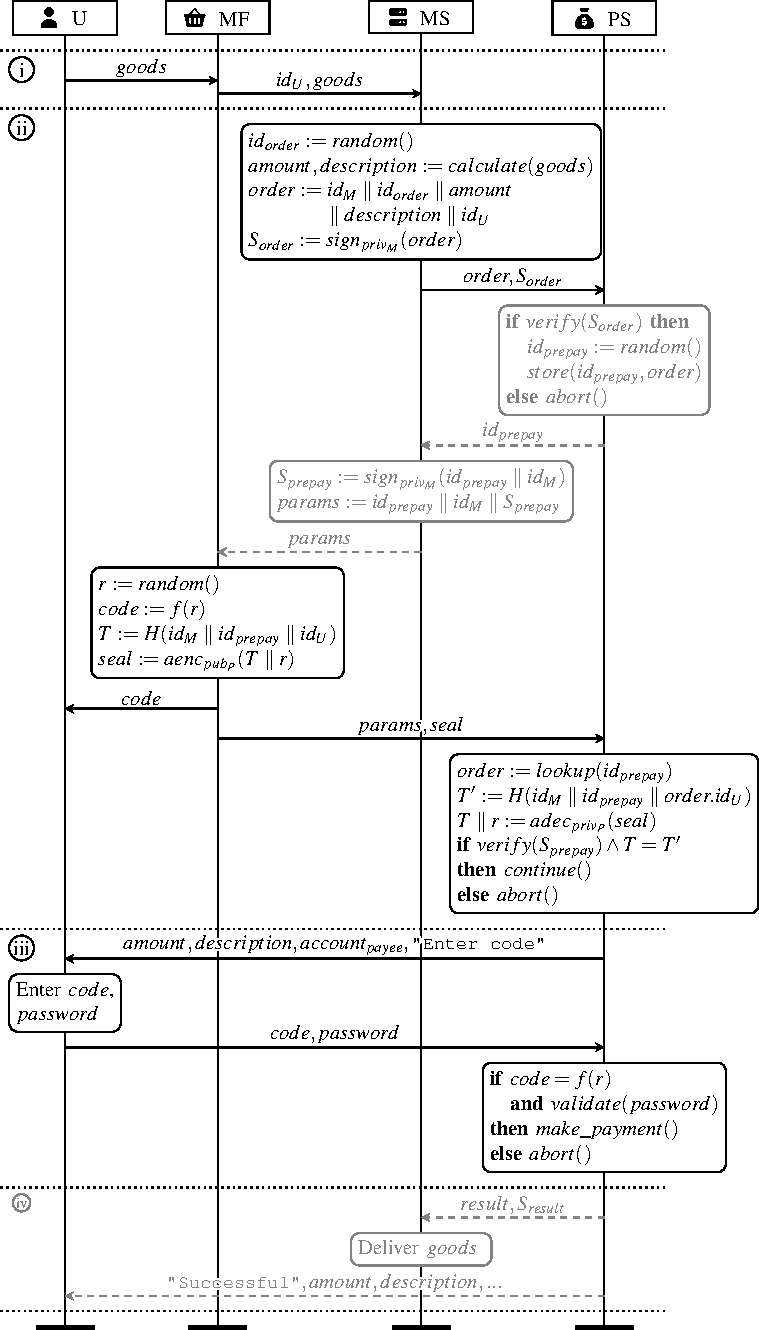
\includegraphics[width=0.85\linewidth]{img/cm_scc.pdf}
  \caption{Sealed Checkout Code on top of payment pattern~B.
    Black elements are new or changed; gray elements are identical to pattern~B.
    Notation: $D$ denotes the fulfilment target of the order; $H$ denotes a hash function; $aenc_{k}(m)$ and $adec_{k}(c)$ denote public-key encryption and decryption; $f$ maps a nonce to a short code; $lookup(id_{prepay})$ returns the order that \emph{PS} recorded for $id_{prepay}$.}
  \label{fig:cm_scc}
\end{figure}

SCC uses the user as the link between \emph{MF} and \emph{PS} that the attacker does not control.
For each payment, \emph{MF} draws a fresh nonce $r$, seals it to \emph{PS} together with a digest of the order handle and the fulfilment target, and shows a short code derived from $r$ to the user.
\emph{PS} opens the seal only for the order it was created for, and completes the payment only if the user enters the same code.
Fig.~\ref{fig:cm_scc} shows the workflow on top of payment pattern~B.

\textbf{Fulfilment target.}
The fulfilment target $D$ is the information that determines who receives the goods, such as a shipping address, a recipient, a mobile number to top up, or a game account.
The user enters or selects $D$ in \emph{MF} at checkout, so the value held by \emph{MF} comes from the user over a secure channel.

\textbf{Order Phase.}
The user selects $goods$ and $D$ in \emph{MF}, and \emph{MF} sends $id_{U}$, $goods$, and $D$ to \emph{MS}.

\textbf{Prepayment Phase.}
\emph{MS} includes $D$ in the order it signs and submits to \emph{PS}, and \emph{PS} records the order under a fresh $id_{prepay}$.
\emph{MS} then generates the payment parameters exactly as in pattern~B.
Upon receiving the parameters, \emph{MF} draws $r$, computes $code = f(r)$ and $T = H(id_{M} \parallel id_{prepay} \parallel D)$ with the $D$ entered by the user, and encrypts $T \parallel r$ under the public key $pub_{P}$ of \emph{PS} to obtain $seal$.
\emph{MF} displays $code$ to the user and sends the payment parameters together with $seal$ to \emph{PS}.
\emph{PS} verifies $S_{prepay}$, looks up the order recorded for $id_{prepay}$, recomputes $T'$ from the merchant identifier, the order handle, and the fulfilment target in that order, and decrypts $seal$.
It continues only if $T = T'$.

\textbf{Authorization Phase.}
\emph{PS-App} displays the amount, the description, and the payee account, and asks the user to enter the code.
The user enters the code shown by \emph{MF} together with the payment password, and \emph{PS} completes the payment only if the code equals $f(r)$ and the password is valid.

\textbf{Notification Phase.}
This phase is identical to pattern~B, and \emph{MS} fulfils the order to $D$.

\textbf{Direction of the code.}
\emph{PS} never displays the code.
Payment parameters are bearer tokens: any party holding them can open the cashier.
If \emph{PS-App} displayed the code for the user to compare, an attacker that intercepts the parameters and the seal could open the cashier under its own payment account, read the code, and choose a nonce $r_A$ with $f(r_A)$ equal to that code for its own order.
In SCC the code travels only from \emph{MF} to the user and from the user to \emph{PS}, both over secure channels.

\textbf{Integration.}
Merchants integrate SCC by adding $D$ to the signed order.
The seal and the code are computed by the payment SDK embedded in \emph{MF}, which also carries $pub_{P}$, and the prepayment and notification interfaces remain unchanged.

\subsection{Security Analysis}

The attacker controls \emph{MF} $\Longleftrightarrow$ \emph{MS} and \emph{MF} $\Longleftrightarrow$ \emph{PS} and obtains legitimate payment parameters for its own orders through the order oracle.
To make the user pay for an order of its own, the attacker has three options.

\begin{enumerate}[leftmargin=*]
  \item \textbf{Substitute its own order.}
  The attacker replaces the user's payment parameters with those of its own order, either on \emph{MF} $\Longleftrightarrow$ \emph{MS} (Variant~\Rom{1}) or on \emph{MF} $\Longleftrightarrow$ \emph{PS} while keeping the user's seal (Variant~\Rom{2}).
  In Variant~\Rom{1}, \emph{MF} seals the attacker's order handle together with the user's $D$; in Variant~\Rom{2}, the seal carries the user's order handle.
  \emph{PS} recomputes $T'$ from the attacker's order, which carries the attacker's own handle and fulfilment target, so $T \neq T'$ and \emph{PS} aborts.
  \item \textbf{Forge a seal for its own order.}
  The attacker builds a consistent seal for its own order with a nonce $r_A$ of its choice.
  \emph{PS} opens the cashier, but the payment requires $f(r_A)$, while the user enters the code $f(r)$ shown by its own \emph{MF}.
  The nonce $r$ appears only inside the seal and as the code on the channel between \emph{MF} and the user, so the attacker can only guess.
  With a four-digit code, a guess succeeds with probability $10^{-4}$, and \emph{PS} bounds the number of failed attempts per payment.
  \item \textbf{Tamper with the fulfilment target.}
  The attacker changes $D$ on its way to \emph{MS}.
  The order at \emph{PS} then carries the attacker's target while \emph{MF} seals the user's target, so $T \neq T'$ and the payment fails.
\end{enumerate}

In every case the attack ends with a failed payment and does not redirect the user's funds or goods.

\subsection{Symbolic Verification}


\begin{table}[t]
\centering
\small
\setlength{\tabcolsep}{5pt}
\renewcommand{\arraystretch}{1.12}

\caption{Verification Results of Countermeasure. \textcolor{xgreen}{\ding{51}}~indicates that the security property is satisfied.}
\label{tab:countermeasure-results}

\begin{tabularx}{\linewidth}{Xccccc  >{\raggedright\arraybackslash}X }
\toprule
\textbf{Protocol} &
\textbf{IA-O1} & \textbf{IA-O2} & \textbf{IA-UA} & \textbf{IA-R1} & \textbf{IA-R2} & \textbf{Time (s)} \\
\midrule

SCC & \textcolor{xgreen}{\ding{51}}  & \textcolor{xgreen}{\ding{51}}  & \textcolor{xgreen}{\ding{51}} & \textcolor{xgreen}{\ding{51}} & \textcolor{xgreen}{\ding{51}}  & 454.94\\

\bottomrule
\end{tabularx}

\end{table}

We model SCC in \Tamarin following the countermeasure models of our artifact, with the same channel rules, query oracle, tactics, and lemmas.
The model uses the Base assumption, in which both \emph{MF} $\Longleftrightarrow$ \emph{MS} and \emph{MF} $\Longleftrightarrow$ \emph{PS} are insecure; it grants the attacker the capabilities of both SecureMS and SecurePS.
Through the order oracle, the attacker places orders with arbitrary amounts and descriptions on its own account, and each such order carries the attacker's own fulfilment target, consistent with the merchant's record of the order.

The user commits to the order when the payment completes, because \emph{PS} checks the code after the user submits it.
To confirm that this commit point preserves the discriminating power of IA-O2, we applied the same change to all six protocols of Table~\ref{tab:lemma-results} under all three channel assumptions; IA-O2 remains falsified in all 18 models.

Table~\ref{tab:countermeasure-results} summarizes the results.
SCC satisfies all five security properties under the Base assumption.
The verification used \Tamarin version~1.10.0 on a server with 32 CPU cores and 187~GB of memory (peak usage 7.0~GB).

%-------------------------------------------------------------------------------
\subsection{Discussion}
%-------------------------------------------------------------------------------

In this paper, we identify a novel variant of order tampering attacks through formal analysis and demonstrate the attack in real-world payment systems.
Our findings reveal a long-standing anti-pattern in the high-level protocol design of third-party online payment systems, namely the absence of user-side order authentication.
To address this issue, we propose a new payment model that systematically eliminates this design deficiency.

\textbf{Advantages.}
From a protocol design perspective, our payment model exhibits three key advantages.
\begin{enumerate}
  \item \textcolor{red}{\textbf{Minimal trust reduction.}}
At the design level, we reduce reliance on trusted external channels, ensuring payment security even under the weakened external channel assumption.
  \item \textcolor{red}{\textbf{Backward compatibility.}}
Our payment model is highly compatible with existing payment models, preserving their four-phase structure and facilitating incremental deployment and adoption by payment service providers.
  \item \textbf{Formally provable security.} 
Our formal analysis results demonstrate that our payment model effectively prevents order tampering attacks during regular payments and satisfies all security properties defined in this paper.
\end{enumerate}

\textbf{Limitations.} 
We honestly present the limitations and trade-offs of our payment model.
\begin{enumerate}
  \item \textbf{Signature and storage overhead.}
Our payment model introduces one additional signature operation, and requires both merchants and users to locally store extra keys, which incurs additional computational and implementation overhead.
However, no new cryptographic primitives are introduced, and we consider the resulting overhead to be acceptable in practice.
  \item \textbf{Additional user interaction during the initial payment.}
During the initial payment, users are required to explicitly confirm their trust in the merchant, introducing additional user interaction.
For regular payments, no extra interaction is required, and the overall user experience remains comparable to that of existing payment models.
  \item \textbf{No security improvement for the initial payment.}
Our proposed model does not provide additional security guarantees for the initial payment.
Instead, our design follows the widely adopted Trust-On-First-Use (TOFU) model, under which the initial interaction may be vulnerable to active network attacks.
Once a legitimate payment context is established, however, any subsequent deviation can be reliably detected.
Consequently, while an adversary may interfere with the initial payment, our scheme guarantees the integrity of subsequent payments and enables attack detection even if the first payment was compromised.
\end{enumerate}
%-------------------------------------------------------------------------------
\section{Related Work}
%-------------------------------------------------------------------------------

A paragraph of text goes here. Lots of text. Plenty of interesting
text. Text text text text text text text text text text text text text
text text text text text text text text text text text text text text
text text text text text text text text text text text text text text
text text text text text text text.
More fascinating text. Features galore, plethora of promises.

% 重点不是列文献，而是：

% > No prior work defines payment security as a layered semantic agreement problem.
%-------------------------------------------------------------------------------
\section{Conclusion}
%-------------------------------------------------------------------------------

This paper presents a systematic and hierarchical security modeling, formal verification, and empirical evaluation of the third-party online payment ecosystem, revealing and validating a long-standing yet underestimated design anti-pattern in industrial practice:
the lack of a strong binding between user payment authorization and order semantics, which leads to the widespread prevalence of order tampering attacks.
Under a realistic threat model that no longer assumes all communication channels to be secure, our formal model covers representative platforms (e.g., Alipay and WeChat Pay), typical payment scenarios (in-app payments, mobile web payments, and QR-code-based payments), as well as two mainstream payment models (Model~A and Model~B), 
and employs the Tamarin Prover to formally analyze the security of the underlying protocols.
Our analysis shows that as long as an insecure channel exists between the merchant frontend and the merchant server (MF--MS), or between the merchant frontend and the payment system (MF--PS), there exist feasible order tampering paths that are transferable across different scenarios and payment models.
Our real-world attack reproduction experiments further corroborate this conclusion.
Based on these findings, we propose and formally verify a user-side order authentication mechanism, fundamentally breaking the tampering chain while balancing security and compatibility within the payment workflow.

The main contributions of this paper are as follows:
\begin{enumerate}
  \item \textbf{A unified formal abstraction of third-party online payments.}
    We systematically characterize the roles and interaction boundaries among users, merchant frontends/servers, and payment systems, and abstract three common payment scenarios and two payment models into a unified semantic framework that is reusable for payment protocol security analysis.
  \item \textbf{A general security model for online payments.}
    We define and formalize core security properties surrounding the consistency of orders and payment results, as well as replay resistance, with a particular emphasis on injective agreement, and conduct proofs and counterexample searches for multiple protocol instances under realistic non–fully-secure channel assumptions.
  \item \textbf{Revealing and validating pervasive order tampering attacks.}
    Our formal verification results provide necessary and sufficient conditions for successful attacks when MF--MS or MF--PS channels are insecure. 
    We identify two major attack variants and explain their transferability and reusability across different scenarios and payment models.
  \item \textbf{Reproducing real-world vulnerabilities and quantifying their impact.}
    On the Android platform, we discover that a large number of merchant apps are vulnerable to order hijacking and tampering due to their use of implicit Intents for interacting with payment apps. 
    We successfully carry out attacks and, through large-scale measurements, find that approximately $20\%$ of the evaluated applications are affected, impacting hundreds of millions of users. 
    We further conduct responsible disclosure and facilitate remediation by platforms and merchants.
  \item \textbf{A deployable and formally verified defense \\ mechanism.}
    Our user-side order authentication mechanism binds a user public key at the granularity of user–merchant pairs, tightly coupling payment authorization with order semantics. 
    Under insecure channel assumptions, we formally prove that it satisfies all defined security properties, and discuss its compatibility with existing platforms and its deployment costs.
\end{enumerate}

From a broader perspective, our work offers three important insights for the security research of online payment systems.
First, the security of payment protocols must not rely on idealized assumptions of fully secure channels, but instead explicitly account for cross-application interactions and channel degradation risks inherent in the mobile ecosystem.
Second, consistency around order semantics and explicit endpoint binding are fundamental to payment security.
The absence of such protocol design elements can easily introduce opaque attack surfaces in complex ecosystems.
Third, formal methods and real-world measurements are complementary: the former establishes provable security boundaries, while the latter exposes systemic vulnerabilities in deployment and provides prioritization guidance for remediation and standardization.


%-------------------------------------------------------------------------------
\bibliographystyle{plain}
\bibliography{library}

%%%%%%%%%%%%%%%%%%%%%%%%%%%%%%%%%%%%%%%%%%%%%%%%%%%%%%%%%%%%%%%%%%%%%%%%%%%%%%%%
\end{document}
%%%%%%%%%%%%%%%%%%%%%%%%%%%%%%%%%%%%%%%%%%%%%%%%%%%%%%%%%%%%%%%%%%%%%%%%%%%%%%%%

%%  LocalWords:  endnotes includegraphics fread ptr nobj noindent
%%  LocalWords:  pdflatex acks